\documentclass{article}
\usepackage{tikz}
\usetikzlibrary{angles, quotes}
\usepackage{amssymb}
\usepackage{pgfplots}
\pgfplotsset{width=10cm,compat=1.9}
\usepgfplotslibrary{statistics}
\usepackage[left=2.54cm,right=2.54cm,top=2.54cm,bottom=2.54cm]{geometry}
\usepackage{tasks} %Paquete necesario para la producción de items horizontales para algunos ejercicios de tarea empleando el comando /begin{multicols}}{#}.../end{multicols} para ayudarnos a reducir las páginas
\usepackage{pdflscape} %comando que permite cambiar a orientación horizontal las hojas%
\usepackage{soul} %Paquete para permitir la compilación de acentos usando el comando {\hl{}}}\\
\sethlcolor{yellow(munsell)} %comando para definir el color para el subrayado usando el comando \hl
\usepackage[utf8]{inputenc}
\usepackage[spanish]{babel}
\usepackage{icomma}
\usepackage{ragged2e}		
\usepackage{siunitx}
\usepackage{url}
\usepackage[colorlinks=true, urlcolor=blue,  linkcolor=Cerulean, citecolor=green]{hyperref}
\usepackage{pdfpages}
\usepackage{blindtext} %Paquete que genera texto ficticio (dummy text) con el comando: \blindtext
\usepackage{cancel} %in the preamble gives you four different modes of striking through: \cancel{text to cancel} draws a diagonal line (slash) through its argument, \bcancel{text to cancel} uses the negative slope (a backslash), \xcancel{text to cancel} draws an X (actually \cancel plus \bcancel), \cancelto{〈value〉}{〈expression〉} draws a diagonal arrow through the 〈expression〉pointing to the 〈value〉 (math-mode only)
\usepackage{csquotes}
\usepackage{afterpage}
\usepackage{parskip} 
\usepackage{float}
\usepackage{enumitem}
%\usepackage{multicol}%Paquete que permite la creación aislada de columnas de texto. De esta forma se reduce la cantidad de páginas en nuestro documento
\usepackage{lipsum} %Paquete que genera texto de relleno al igual que \usepackage{blindtext}, se usa con el comando \lipsum[#-#] los #(hashtags) delimitan el número de páginas que deseamos ocupar del paquete lipsum para usarlos como relleno. 

% Definir el comando personalizado para la nota
\newcommand{\mynote}[1]{%
\begin{tikzpicture}[baseline=-0.75ex]
\node[draw, circle, fill=Apple Green!60, inner sep=2pt] (note) {\textbf{Nota:}};
\end{tikzpicture}%
\ \textit{#1}%
}

% Definición de comandos para variables con barra
\newcommand{\xbar}{\overline{x}}
\newcommand{\ybar}{\overline{y}}

\newenvironment{Figura}
{\par\medskip\noindent\minipage{\linewidth}}
{\endminipage\par\medskip}
\usepackage{caption}
\usepackage[
backend=biber,
sorting=none,
url=true
]{biblatex} %bibliografía
\addbibresource{biblio.bib}
% Establecer el espacio entre las entradas de la bibliografía
\setlength{\bibitemsep}{1\baselineskip} % Puedes ajustar el valor según tus preferencias
\usepackage{amsmath,amsthm,amssymb,amsfonts}
\usepackage{pifont} %Permite la compilación del comando \xmark: es el símbolo de la tachita
\usepackage{mathtools} %permite la compilación de símbolos para matrices
\usepackage{empheq} %Paquete que se relaciona con \usepackage[most]{tcolorbox} para la creación de cuadros/cajas de colores para delimitar los resultados matemáticos o líneas de texto usando la línea de comando: \begin{empheq}[box={\mymath[colback=orange(webcolor)!70,drop lifted shadow]}]{equation*} \end{empheq}
\usepackage[most]{tcolorbox} %Paquete que se relaciona con \usepackage{empheq} para la creación de cuadros/cajas de colores para delimitar los resultados matemáticos o líneas de texto
\renewcommand{\qedsymbol}{$\blacksquare$}
\usetikzlibrary{positioning,decorations.pathreplacing} %Paquete que permite la compilación de llaves para cuadros sinópticos (brace diagram) 
\usepackage{schemata} %The schemata package is designed just for these brace diagrams
\usepackage{booktabs}

\newcommand\AB[2]{\schema{\schemabox{#1}}{\schemabox{#2}}} %comando o paquete necesario para crear cuadros sinópticos

\newtcbox{\mymath}[1][]{%
nobeforeafter, math upper, tcbox raise base,
enhanced, colframe=blue!30!black,
colback=blue!30, boxrule=1pt,
#1} %Comando importante para encasillar los resultados matemáticos en cajas de diferentes colores, se relaciona con los paquetes \usepackage{empheq} y \usepackage[most]{tcolorbox} 

\newenvironment{sysmatrix}[1]
{\left(\begin{array}{@{}#1@{}}}
{\end{array}\right)}
\newcommand{\ro}[1]{%
\xrightarrow{\mathmakebox[\rowidth]{#1}}%
}
\newlength{\rowidth}% row operation width
\AtBeginDocument{\setlength{\rowidth}{3em}}  %Comando importante para laproducción de lineas de operaciones entre matrices, método de Gauss o Gauss Jordan se relaciona con \newenvironment{sysmatrix}

%formato para cambiar el horario a español
\usepackage[spanish]{datetime2}
\DTMsetdatestyle{spanish}

\renewcommand{\today}{\DTMdisplaydate{\the\year}{\the\month}{\the\day }{-1}}
%%%%%%%%%%%%%%%%%%%%%%%%%%%%%%%%%%%%%%%%%

\usepackage{datetime}
\newcommand{\mycurrenttime}{\xxivtime}

%%%%%%%%%%%%%%%%%%%%%%%%%%%%%%%%%%%%%%%%%%%%%%%%%%%%%%%%%%%%%%%%%%%%%%%%%%%%%%%%%%%%%%%%%%%%%%%%%%%%%%%%%%%%%%%%%%%%%%%%%%%%%%%%%%%%%%%%%%%%%%%%%


%%%%%%%%%%%%%Caja de color para el título%%%%%%%%%%%%%%%%%%%%%%%%%%%%%%%%%%%%%%%%%%%%%%%%%%%%%%

\definecolor{myframecolor}{RGB}{1, 45, 75} % Prussian Blue
\definecolor{myboxcolor}{RGB}{0, 107, 92} % Apple Green

\newtcolorbox{mybox}{
enhanced,
colback=myboxcolor!7, % Color de fondo del cuadro
colframe=myframecolor, % Color del marco del cuadro
arc=0pt,
boxrule=1pt,
borderline west={2mm}{-10mm}{myframecolor}, % Borde en el lado izquierdo
sharp corners=southwest,
width=\linewidth,
before=\par\vspace{\bigskipamount}, % Espacio antes del cuadro
after=\par\vspace{\bigskipamount} % Espacio después del cuadro
}

%%%%%%%%%%%%%%%%%%%%%%%%%%%%%%%%%%%%%%%%%%%%%%%%%%%%%%%%%Nueva caja%%%%%%%%%%%%%%%%%%%%%%%%%%%%%%%%%%%%%%%%%%%%%%%%%%%%%%%%%%%%%%%%%

\newtcolorbox{mybox2}{
enhanced,
colback=Apple Green!7, % Color de fondo del cuadro
colframe=Apple Green, % Color del marco del cuadro
arc=0pt,
boxrule=1pt,
borderline west={2mm}{-10mm}{Apple Green}, % Borde en el lado izquierdo
sharp corners=southwest,
width=\linewidth,
before=\par\vspace{\bigskipamount}, % Espacio antes del cuadro
after=\par\vspace{\bigskipamount} % Espacio después del cuadro
}


\newcommand{\euler}{e} %Comando para producir letra e de euler
\newenvironment{remark}{\par\vfill\footnotesize % Vertical white space above the remark and smaller font size
\begin{list}{}{
	\leftmargin=80pt % Indentation on the left
	\rightmargin=60pt}\item\ignorespaces % Indentation on the right
\makebox[-2.5pt]{\begin{tikzpicture}[overlay]
		\node[draw=Horizon!60,line width=2.5pt,circle,fill=Horizon!25,font=\sffamily\bfseries,inner sep=4pt,outer sep=0pt] at (-19pt,5pt){\textcolor{Horizon}{Nota}};\end{tikzpicture}} % Blue Nota in a circle
\advance\baselineskip -1pt}{\end{list}\vskip5pt} % Tighter line spacing and white space after remark
\usepackage{graphicx}

\usepackage{titling}

\input{colores.tex}

%%Producir signos de cita textual``Asignatura''

\newcommand{\xmark}{\ding{55}} %%%comando que genera la tachita

\newenvironment{MyColorPar}[1]{%
\leavevmode\color{#1}\ignorespaces%
}{%
}%

%%%%%%%%%%%%%%%%%%% Título de la tarea, Nombre de alumno

\title{ \textcolor{Sun}{\textbf{T1: \textcolor{Cinnabar}{\textbf{Redes}}}}}
\author{\emph{Tarea} $\boldsymbol{\mid}$ \textcolor{Tarawera}{\textbf{Oscilaciones de la red}}}
\date{\today}

%%%%%%%%%%%%%%%%%%% Datos de la Materia

\usepackage{fancyhdr}
\fancypagestyle{plain}{%  the preset of fancyhdr 
\fancyhf{} % clear all header and footer fields
\fancyfoot[R]{
\includegraphics[width=2cm]{LogoFCFMBUAP (1).png}}
\fancyfoot[L]{{\bfseries{\thedate{}}} a las {\bfseries{\mycurrenttime{}}} horas{} (GMT-6, H. Puebla de Zaragoza, Pue)}
\fancyhead[L]{\textbf{Asignatura:} Estado Sólido}
\fancyhead[R]{\theauthor}
}
\makeatletter
\def\@maketitle{%
\newpage
\null%
\begin{center}%
\let \footnote \thanks
{\LARGE \@title \par}%
\vskip 1em%
%{\large \@date}%
\end{center}%
}
\makeatother

\usepackage{lipsum}  
\usepackage{cmbright}


%%%%%%%%%%%%%%%%%%%%%%%%%%%%%%%%%%%%%%%%%%%%%%%%%%%%%%%%%%%%%%%%%%%%%%%%%%%%%%%%%%%%%%%%%%%%%%%%%%%%%%%%%%%%%%%%%%%%%%%%%%%%%%%%%%%%%%%%%%%%%%%%%%%%%%%%%%%%%%%%%%%%%%%%%%%%%%%%%%%%%%%%%%%%%%%%%%%%%%

% Por si el color se llama "Apple Green" con espacio en colores.tex:
\colorlet{AppleGreen}{Apple Green}

% Caja AppleGreen con tono ajustable
\newenvironment{AGbox}[1][7]% 7 = tono por defecto (más grande => más claro)
{%
  \begin{tcolorbox}[
    enhanced, breakable,
    colframe=AppleGreen,
    colback=AppleGreen!#1,
    boxrule=1pt,
    borderline west={2mm}{-10mm}{AppleGreen},
    sharp corners=southwest,
    left=14pt,right=14pt,top=10pt,bottom=10pt,
     boxsep=6pt,
  ]%
}{%
  \end{tcolorbox}%
}


\begin{document}



\maketitle

%%%%%%%%%%%%%%%%%%% Datos del profesor, campus, aula e integrantes

\begin{mybox2}
\noindent
\begin{tabular}{@{}p{3.7cm}p{10.4cm}@{}}
\textbf{Profesor} & Dra. Ana Lilia González Ronquillo \\[3pt]
\textbf{Campus / Facultad} & \textcolor{prussianblue}{\textbf{C.U. BUAP}} / \textcolor{trueblue}{\textbf{FCFM}} \\[3pt]
\textbf{Edificio / Salón} & \textcolor{prussianblue}{\textbf{FM9}} / \textcolor{trueblue}{\textbf{301}} \\[6pt]
\textbf{Alumno} & Julio Alfredo Ballinas García
\end{tabular}
\end{mybox2}
\vspace{1cm}


\vspace{0.5cm}
\begin{center}
\begin{tikzpicture}
	% Dibuja círculos rellenos en diferentes colores
	\fill[bittersweet] (0,0) circle (0.17cm);
	\fill[Apple Green] (0.6,0) circle (0.17cm);
	\fill[trueblue] (1.2,0) circle (0.17cm);
	\fill[Aguamarina] (1.8,0) circle (0.17cm);
	\fill[Sun] (2.4,0) circle (0.17cm);
	\fill[orange(colorwheel)] (3.0,0) circle (0.17cm);
	\fill[Pesto] (3.6,0) circle (0.17cm);
	\fill[blue-violet] (4.2,0) circle (0.17cm);
	\fill[ticklemepink] (4.8,0) circle (0.17cm);
	\fill[Gallery] (5.4,0) circle (0.17cm);
	\fill[Mantle] (6.0,0) circle (0.17cm);
	\fill[Nevada] (6.6,0) circle (0.17cm);
	\fill[onyx] (7.2,0) circle (0.17cm);
	% Agrega más círculos o modifica los colores según sea necesario
\end{tikzpicture}
\end{center}  \vspace{0.5cm}

\section*{\textcolor{Tarawera}{\textbf{Lista de problemas y soluciones}}}
\addcontentsline{toc}{section}{\textcolor{Tarawera}{\textbf{Problemas: cap 3}}}

\setlength{\columnsep}{2cm}
%\begin{multicols}{2}
%=============================
% PR. 1.1 — Estructura cúbica simple (SC)
%=============================
\begin{AGbox}[8]
\begin{enumerate}[label={{\textcolor{trueblue}{\textbf{Pr.} \arabic*.1}}}, start=1]
  \item Use el modelo de esferas duras para mostrar que el factor de empaquetamiento de una estructura \textbf{cúbica simple (SC)} es de 0.52. Esto significa que el 52\% del volumen de la celda unitaria está ocupado por átomos, mientras que el 48\% restante corresponde a espacios vacíos
\end{enumerate}
\end{AGbox}

\vspace{0.5cm}
\textcolor{Cinnabar}{\textbf{Solución:}}

\begin{figure}[H]
  \centering
  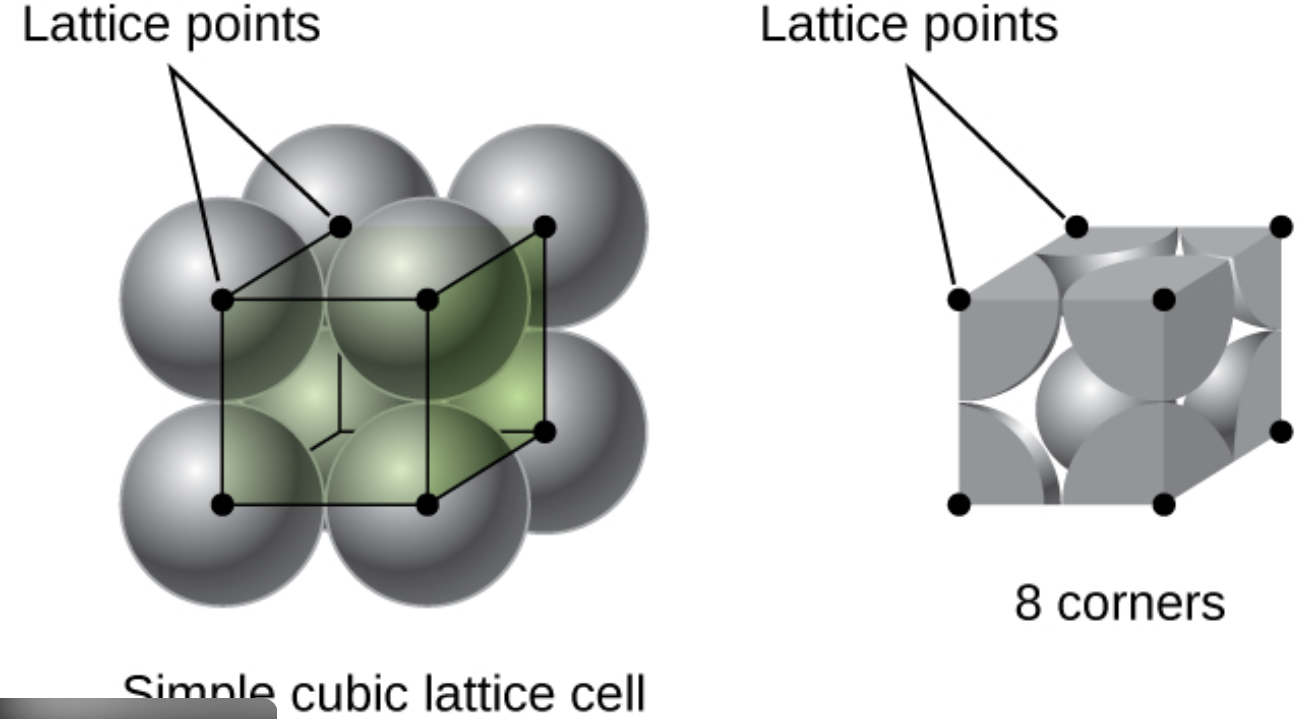
\includegraphics[width=0.50\textwidth]{sc.png}
  \caption{\textbf{Estructura cúbica simple (SC).} Los centros atómicos ocupan las 8 esquinas del cubo. En esta estructura, las esferas vecinas se tocan únicamente a lo largo de la arista: si consideramos dos esquinas adyacentes, la distancia entre sus centros es igual a la longitud de la arista \(a\), y el contacto implica que esa distancia coincide con el diámetro atómico \(2r\); de ahí que \(a=2r\). Cada átomo ubicado en una esquina está compartido por 8 celdas adyacentes, por lo que cada una de ellas sólo contiene una fracción \(1/8\) de ese átomo. Al sumar todas las contribuciones, el número \textbf{efectivo de átomos por celda unitaria} es \(N_{\text{ef}}=8\times\tfrac{1}{8}=1\). Este valor indica que, aunque hay ocho posiciones de red en las esquinas, el contenido real equivalente dentro de una celda cúbica simple corresponde a un solo átomo} \label{fig:sc}
\end{figure}


\begin{figure}[H]
  \centering
  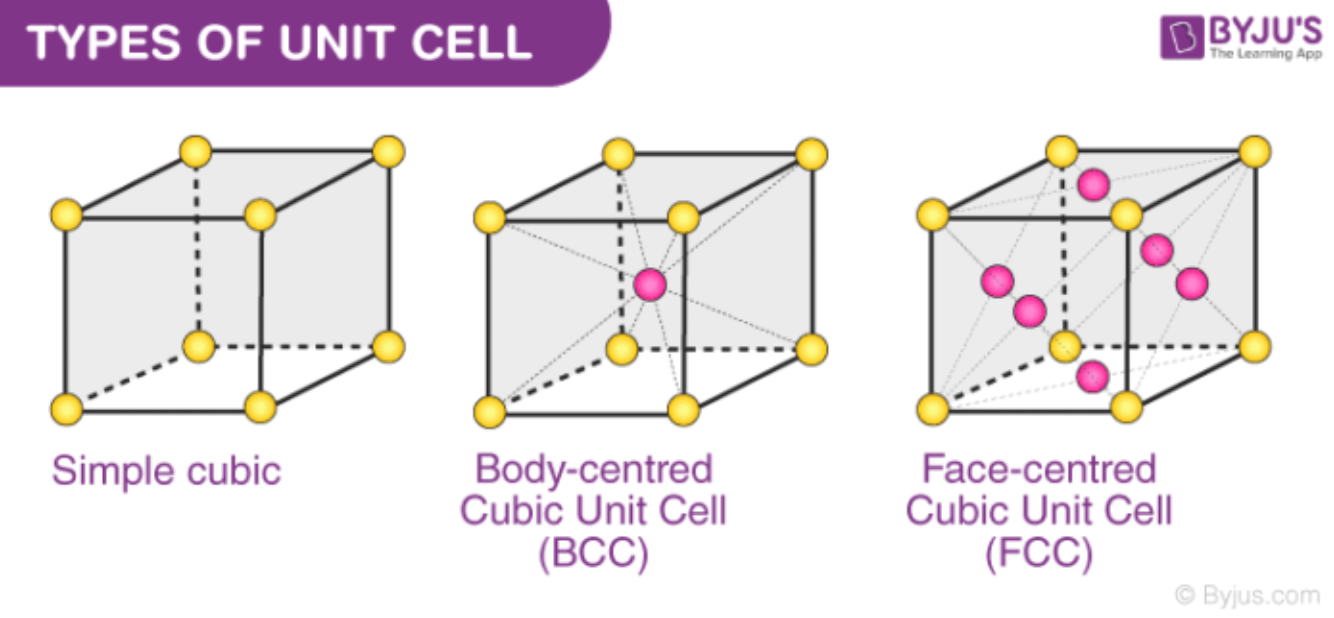
\includegraphics[width=0.50\textwidth]{uc.png}
  \caption{\textbf{Vista de celda unitaria SC con puntos de red.} Los centros en \((0,0,0)\) y \((a,0,0)\) ilustran un par de esferas vecinas que se tocan sobre la arista \(\overline{AB}\). La distancia entre centros es \(\lvert (a,0,0)-(0,0,0)\rvert=a\), que debe coincidir con el diámetro \(2r\). Esta observación fija la relación \(a=2r\)}\label{fig:uc}
\end{figure}

El \textcolor{Cerulean}{\textbf{factor de empaquetamiento}} es una medida geométrica que nos indica qué fracción del volumen total de la celda unitaria está realmente ocupada por los átomos, asumiendo que cada átomo se comporta como una \textit{esfera dura}, es decir, que no se deforma y que sólo puede hacer contacto con sus vecinos tangencialmente.  
Matemáticamente, se define como:

\begin{equation}
\begin{split}
\eta &= \frac{V_{\text{átomos en la celda}}}{V_{\text{celda}}}
\end{split} \label{eq:def-factor}
\end{equation}

donde \(V_{\text{átomos en la celda}}\) representa el volumen total ocupado por los átomos contenidos efectivamente dentro de la celda unitaria, mientras que \(V_{\text{celda}}\) corresponde al volumen completo de dicha celda.

Para calcular el numerador debemos saber cuántos átomos contiene realmente la celda, pero considerando que los átomos en las esquinas se \emph{comparten} con otras celdas adyacentes.  
A este conteo se le llama \textbf{número efectivo de átomos por celda unitaria}, y se denota como \(N_{\text{ef}}\).  
En la estructura cúbica simple (SC) hay ocho átomos, uno en cada esquina del cubo, pero cada átomo en una esquina pertenece simultáneamente a ocho celdas vecinas.  
Por lo tanto, cada uno aporta solo una fracción \(1/8\) de su volumen a la celda que estamos analizando.  
Al sumar las contribuciones de todas las esquinas, se obtiene:

\begin{equation}
\begin{split}
N_{\text{ef}} &= 8\times \frac{1}{8} = 1
\end{split} \label{eq:nef-sc}
\end{equation}

Esto significa que, aunque visualmente se vean ocho esferas, el contenido real de materia dentro de una celda cúbica simple equivale a un solo átomo completo.

El volumen total de esos átomos dentro de la celda está dado entonces por el número efectivo multiplicado por el volumen de una esfera de radio \(r\):

\begin{equation}
\begin{split}
V_{\text{átomos en la celda}} &= N_{\text{ef}}\;\frac{4}{3}\pi r^{3}
\end{split} \label{eq:vol-atomos}
\end{equation}

El volumen de la celda cúbica, por su parte, depende únicamente del parámetro de red \(a\), que corresponde a la longitud de la arista del cubo:

\begin{equation}
\begin{split}
V_{\text{celda}} &= a^{3}
\end{split} \label{eq:vol-celda}
\end{equation}

Para poder relacionar ambas magnitudes, necesitamos establecer cómo se vincula el parámetro de red \(a\) con el radio atómico \(r\).  
En la estructura cúbica simple, el contacto entre esferas ocurre \emph{a lo largo de la arista del cubo}.  
Si consideramos dos átomos ubicados en las posiciones \((0,0,0)\) y \((a,0,0)\), la distancia entre sus centros es precisamente \(a\).  
Como las esferas se tocan, esa distancia coincide con el diámetro atómico \(2r\).  
De este modo se obtiene la relación fundamental:

\begin{equation}
\begin{split}
a &= 2r
\end{split} \label{eq:a2r}
\end{equation}

Esta relación geométrica expresa que el parámetro de red es exactamente igual al doble del radio atómico, lo cual tiene sentido visualmente si imaginamos las esferas alineadas sobre la arista, tocándose entre sí.

Ahora sustituimos las expresiones anteriores en la definición \eqref{eq:def-factor}.  
Sustituyendo \(N_{\text{ef}}\) de \eqref{eq:nef-sc}, el volumen atómico de \eqref{eq:vol-atomos}, el volumen de la celda de \eqref{eq:vol-celda} y la relación \(a=2r\) de \eqref{eq:a2r}, tenemos:

\begin{equation}
\begin{split}
\eta &= \frac{N_{\text{ef}}\;\frac{4}{3}\pi r^{3}}{a^{3}}
     \;=\; \frac{1\times \frac{4}{3}\pi r^{3}}{(2r)^{3}}
\end{split} \label{eq:eta-paso1}
\end{equation}

Desarrollamos el denominador y simplificamos los términos en \(r^{3}\):

\begin{equation}
\begin{split}
\eta &= \frac{\frac{4}{3}\pi r^{3}}{8r^{3}}
     \;=\; \frac{4\pi}{3}\cdot\frac{1}{8}
     \;=\; \frac{\pi}{6}
\end{split} \label{eq:eta-paso2}
\end{equation}

Este resultado analítico puede expresarse numéricamente como:

\begin{equation}
\begin{split}
\eta_{\text{SC}} &= \frac{\pi}{6} \approx 0.5236 \approx \boxed{0.52}
\end{split} \label{eq:eta-sc-num}
\end{equation}

El valor \(\eta_{\text{SC}}\) representa el \textcolor{Cerulean}{\textbf{factor de empaquetamiento}} específico de la estructura cúbica simple, e indica que aproximadamente el \(52\%\) del volumen total de la celda unitaria está ocupado por materia sólida (átomos), mientras que el \(48\%\) restante corresponde a espacios vacíos o huecos intersticiales.  
Por esta razón, la estructura SC se considera una de las menos compactas entre las cúbicas.

A partir de este resultado, también se puede definir la \textbf{fracción de huecos} o porosidad geométrica del modelo como:

\begin{equation}
\begin{split}
\phi &= 1 - \eta_{\text{SC}} = 1 - \frac{\pi}{6}
\end{split} \label{eq:porosidad}
\end{equation}







\begin{AGbox}[8]
\begin{enumerate}[label={{\textcolor{trueblue}{\textbf{Pr.} \arabic*.2}}}, start=2]
  \item Use el modelo de esferas duras para mostrar que el factor de empaquetamiento de una estructura \textbf{cúbica centrada en el cuerpo (BCC)} es de 0.68
\end{enumerate}
\end{AGbox}

\vspace{0.5cm}
\textcolor{Cinnabar}{\textbf{Solución:}}

\begin{figure}[H]
  \centering
  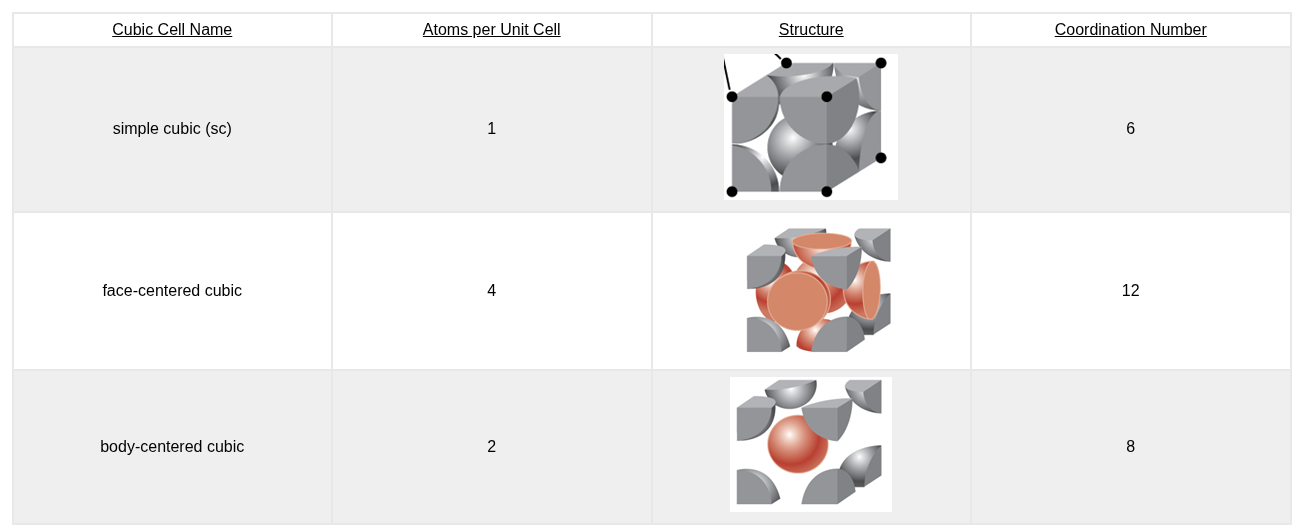
\includegraphics[width=0.70\textwidth]{bcc_tabla.png}
  \caption{\textbf{Celdas cúbicas y número de coordinación.} En la estructura cúbica centrada en el cuerpo (BCC) cada vértice del cubo está ocupado por un átomo, al igual que el centro del cubo. Este último se encuentra completamente contenido dentro de la celda. El número de coordinación de esta red es \(8\), ya que cada átomo del centro está en contacto con los ocho átomos de las esquinas. En la figura se comparan los tres tipos de celdas cúbicas (SC, BCC y FCC) para visualizar sus diferencias de empaquetamiento y contenido atómico} \label{fig:bcc-tabla}
\end{figure}

\begin{figure}[H]
  \centering
  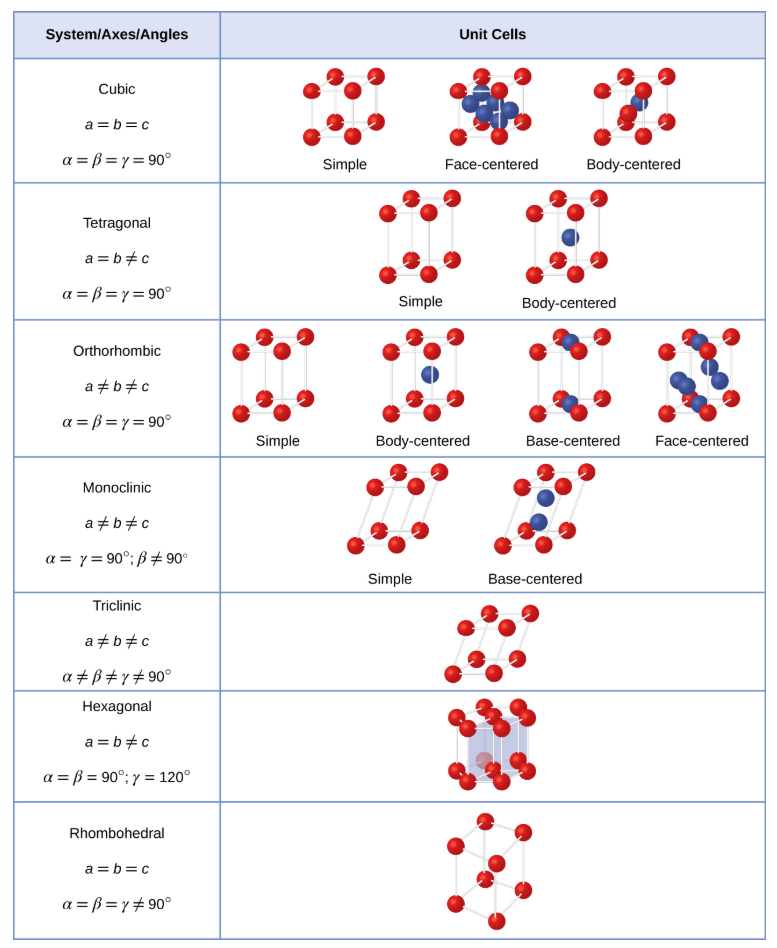
\includegraphics[width=0.70\textwidth]{unit_cells_table.png}
  \caption{\textbf{Vista tridimensional de la celda BCC.} El átomo central se encuentra completamente dentro de la celda, mientras que los de las esquinas se comparten con ocho celdas vecinas. El contacto entre esferas ocurre a lo largo de la \textit{diagonal del cuerpo}: al unir el centro de una esquina con el átomo del centro y continuar hasta la esquina opuesta, se forma una diagonal de longitud \(\sqrt{3}\,a\). En ella caben cuatro radios atómicos, lo que establece la relación geométrica \(a = \tfrac{4r}{\sqrt{3}}\)} \label{fig:bcc-sistemas}
\end{figure}

El \textcolor{Cerulean}{\textbf{factor de empaquetamiento}} en una red cúbica centrada en el cuerpo (BCC) indica qué proporción del volumen total de la celda unitaria está efectivamente ocupada por los átomos, asumiendo que estos se comportan como esferas duras en contacto.  
Se define de la misma forma general que antes:

\begin{equation}
\begin{split}
\eta &= \frac{V_{\text{átomos en la celda}}}{V_{\text{celda}}}
\end{split} \label{eq:def-factor-bcc}
\end{equation}

donde \(V_{\text{átomos en la celda}}\) representa el volumen total aportado por los átomos efectivamente contenidos dentro de la celda unitaria, y \(V_{\text{celda}}\) corresponde al volumen geométrico del cubo.

Para calcular el numerador debemos determinar el \textbf{número efectivo de átomos por celda unitaria}, \(N_{\text{ef}}\).  
En la estructura BCC hay ocho átomos ubicados en las esquinas, que se comparten entre ocho celdas vecinas, y un átomo completamente dentro del cuerpo del cubo, que pertenece exclusivamente a esa celda.  
Por tanto, el número efectivo se calcula como:

\begin{equation}
\begin{split}
N_{\text{ef}} &= 8\times\frac{1}{8} + 1 = 2
\end{split} \label{eq:nef-bcc}
\end{equation}

Esto significa que, aunque visualmente hay nueve átomos asociados a cada celda (ocho en los vértices y uno al centro), el contenido real equivalente dentro de una celda unitaria BCC es de dos átomos completos.

El volumen total que ocupan estos átomos se expresa como:

\begin{equation}
\begin{split}
V_{\text{átomos en la celda}} &= N_{\text{ef}}\;\frac{4}{3}\pi r^{3}
\end{split} \label{eq:vol-atomos-bcc}
\end{equation}

Mientras que el volumen de la celda cúbica es:

\begin{equation}
\begin{split}
V_{\text{celda}} &= a^{3}
\end{split} \label{eq:vol-celda-bcc}
\end{equation}

Para poder relacionar \(a\) con el radio atómico \(r\), es necesario identificar la línea a lo largo de la cual se produce el contacto entre esferas.  
En este tipo de red, las esferas no se tocan por las aristas (como en SC) ni por las diagonales de las caras (como en FCC), sino a lo largo de la \textbf{diagonal del cuerpo del cubo}.  
Esta diagonal une dos esquinas opuestas pasando por el átomo central.  
Geométricamente, su longitud está dada por:

\begin{equation}
\begin{split}
d_{\text{cuerpo}} &= \sqrt{3}\,a
\end{split} \label{eq:diag-cuerpo}
\end{equation}

A lo largo de esta diagonal se alinean tres átomos en contacto: uno en cada extremo y el del centro.  
En consecuencia, sobre la diagonal caben cuatro radios atómicos (dos correspondientes a los átomos de las esquinas y dos al átomo del cuerpo).  
Por tanto, la distancia total es:

\begin{equation}
\begin{split}
\sqrt{3}\,a &= 4r
\end{split} \label{eq:contacto-bcc}
\end{equation}

De donde se obtiene la relación entre el parámetro de red y el radio atómico:

\begin{equation}
\begin{split}
a &= \frac{4r}{\sqrt{3}}
\end{split} \label{eq:a-r-bcc}
\end{equation}

Sustituyendo ahora las ecuaciones \eqref{eq:nef-bcc}, \eqref{eq:vol-atomos-bcc}, \eqref{eq:vol-celda-bcc} y \eqref{eq:a-r-bcc} en la definición general \eqref{eq:def-factor-bcc}, se tiene:

\begin{equation}
\begin{split}
\eta &= \frac{N_{\text{ef}}\;\frac{4}{3}\pi r^{3}}{a^{3}}
     = \frac{2\;\frac{4}{3}\pi r^{3}}{\left(\frac{4r}{\sqrt{3}}\right)^{3}}
\end{split} \label{eq:eta-bcc-1}
\end{equation}

Desarrollamos el denominador \(\left(\tfrac{4r}{\sqrt{3}}\right)^{3}=\tfrac{64r^{3}}{3\sqrt{3}}\), cancelamos los factores de \(r^{3}\) y simplificamos:

\begin{equation}
\begin{split}
\eta &= \frac{\frac{8\pi}{3}}{\frac{64}{3\sqrt{3}}}
     = \frac{8\pi}{3}\cdot\frac{3\sqrt{3}}{64}
     = \frac{\pi\sqrt{3}}{8}
\end{split} \label{eq:eta-bcc-2}
\end{equation}

Finalmente, su valor numérico es:

\begin{equation}
\begin{split}
\eta_{\text{BCC}} &= \frac{\pi\sqrt{3}}{8} \approx 0.680
\end{split} \label{eq:eta-bcc-num}
\end{equation}

El valor obtenido \(\eta_{\text{BCC}}\approx0.68\) significa que el \(68\%\) del volumen total de la celda unitaria está ocupado por materia, y el \(32\%\) restante corresponde a huecos intersticiales.  
En comparación con la estructura cúbica simple, la BCC presenta una disposición más densa, ya que incorpora un átomo adicional en el centro del cubo, aumentando así la eficiencia de empaquetamiento.  
Sin embargo, sigue siendo menos compacta que la estructura cúbica centrada en las caras (FCC), que alcanza un valor de \(\eta_{\text{FCC}}\approx0.74\).  
Esto establece que el tipo de contacto entre átomos —en este caso, a lo largo de la diagonal del cuerpo— es el responsable directo del aumento en la forma más compacta del empaquetamiento.


\begin{AGbox}[8]
\begin{enumerate}[label={{\textcolor{trueblue}{\textbf{Pr.} \arabic*.3}}}, start=3]
  \item Use el modelo de esferas duras para mostrar que el factor de empaquetamiento de una estructura \textbf{cúbica centrada en las caras (FCC)} es de 0.74
\end{enumerate}
\end{AGbox}

\vspace{0.5cm}
\textcolor{Cinnabar}{\textbf{Solución:}}

\begin{figure}[H]
  \centering
  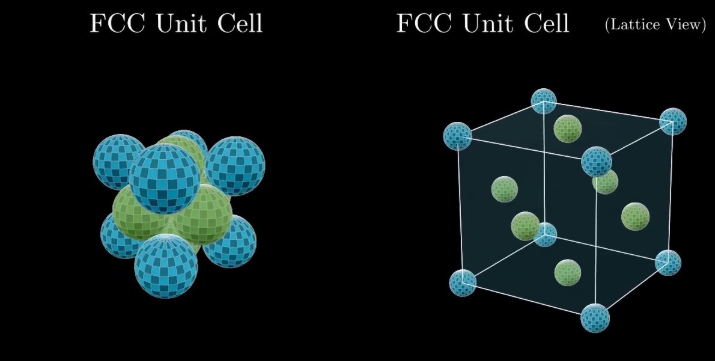
\includegraphics[width=0.70\textwidth]{fcc_celda.png}
  \caption{\textbf{Estructura cúbica centrada en las caras (FCC).} En esta red, los átomos se localizan en los ocho vértices del cubo y en el centro de cada una de sus seis caras. Los átomos de las esquinas se comparten entre ocho celdas, mientras que los ubicados en las caras son compartidos entre dos. El contacto entre esferas se produce a lo largo de la diagonal de una cara, como se indica en el esquema, lo que lleva a la relación geométrica \(a = 2\sqrt{2}\,r\)} \label{fig:fcc-celda}
\end{figure}

\begin{figure}[H]
  \centering
  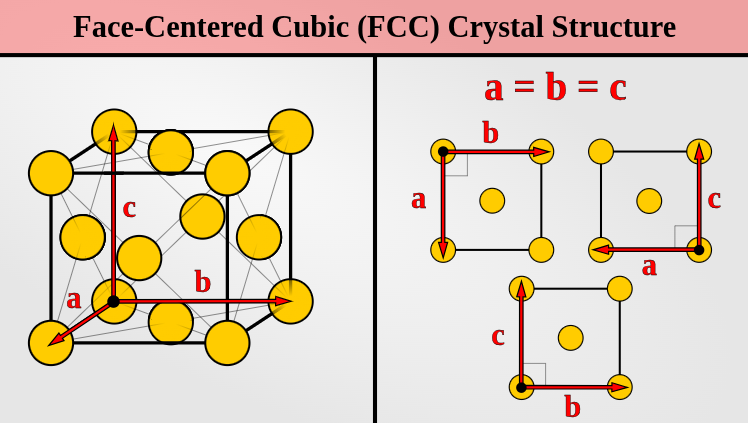
\includegraphics[width=0.70\textwidth]{fcc_contacto.png}
  \caption{\textbf{Vista de la diagonal de cara en la celda FCC.} Al observar una de las caras del cubo, se identifican tres átomos en contacto directo: uno en cada esquina y otro en el centro de la cara. A lo largo de esa diagonal se alinean cuatro radios atómicos, de manera que \(\sqrt{2}\,a = 4r\). Esta relación es la base para determinar el parámetro de red en función del radio atómico} \label{fig:fcc-contacto}
\end{figure}


El \textcolor{Cerulean}{\textbf{factor de empaquetamiento}} en la estructura cúbica centrada en las caras (FCC) representa, al igual que en los casos anteriores, la fracción del volumen total de la celda unitaria que está ocupada por los átomos, idealizados como esferas duras en contacto perfecto.  
Matemáticamente, se expresa de forma general como:

\begin{equation}
\begin{split}
\eta &= \frac{V_{\text{átomos en la celda}}}{V_{\text{celda}}}
\end{split} \label{eq:def-factor-fcc}
\end{equation}

donde \(V_{\text{átomos en la celda}}\) corresponde al volumen total que aportan los átomos efectivamente contenidos dentro de la celda unitaria, y \(V_{\text{celda}}\) representa el volumen geométrico del cubo de parámetro de red \(a\).

Siguiendo la misma metodología que en los casos de la \textbf{estructura cúbica simple (SC)} y la \textbf{centrada en el cuerpo (BCC)}, determinamos primero el número de átomos que componen efectivamente la celda.  
Este número, denominado \textbf{número efectivo de átomos por celda unitaria} \(N_{\text{ef}}\), considera las fracciones de cada átomo que pertenecen a la celda debido a que muchos se comparten con celdas vecinas.


\begin{figure}[H]
  \centering
  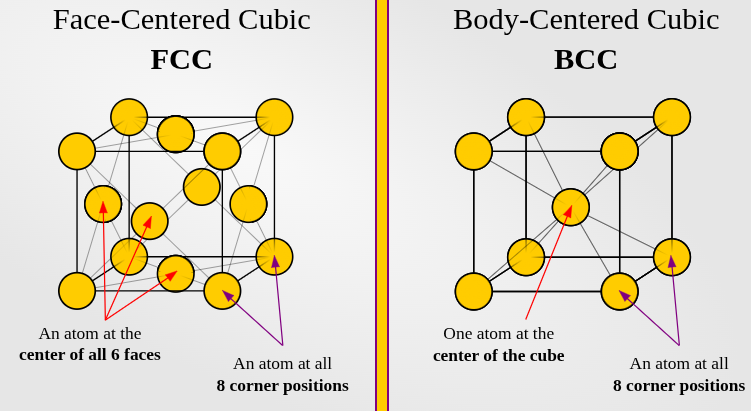
\includegraphics[width=0.50\textwidth]{compar.png}
 \caption{\textbf{Comparación entre las estructuras cúbicas centradas en las caras (FCC) y centradas en el cuerpo (BCC).}  
En la red \textbf{BCC} (a la derecha) los átomos se localizan en las ocho esquinas y en el centro del cubo, donde este último está completamente contenido dentro de la celda y en contacto con los ocho átomos de los vértices a lo largo de la diagonal del cuerpo.  
En la estructura \textbf{FCC} (a la izquierda), los átomos también ocupan las ocho esquinas, pero además se ubican en el centro de cada una de las seis caras del cubo, compartiéndose entre dos celdas vecinas.  
El contacto entre átomos en FCC ocurre a lo largo de las diagonales de las caras, lo que da lugar a un empaquetamiento más compacto (\(\eta_{\text{FCC}}=0.74\)) en comparación con la estructura BCC (\(\eta_{\text{BCC}}=0.68\)).  
Esta diferencia geométrica explica por qué, aunque ambas pertenecen al sistema cúbico, la FCC logra una mayor densidad de empaque.}
 \label{fig:fcc-compar}
\end{figure}

En FCC hay:

\begin{itemize}
\item[$\bullet$] 8 átomos en las esquinas, cada uno compartido entre 8 celdas (\(1/8\) de contribución), y  
\item[$\bullet$] 6 átomos ubicados en el centro de cada cara, cada uno compartido con 2 celdas (\(1/2\) de contribución).  
\end{itemize}

Por tanto, el número efectivo resulta en lo siguiente:

\begin{equation}
\begin{split}
N_{\text{ef}} &= 8\times\frac{1}{8} + 6\times\frac{1}{2} = 4
\end{split} \label{eq:nef-fcc}
\end{equation}

Esto significa que, aunque visualmente se perciben 14 posiciones atómicas asociadas a cada celda (8 vértices y 6 centros de cara), el contenido real de materia dentro de la celda unitaria equivale a cuatro átomos completos.

El volumen total que ocupan dichos átomos puede escribirse como:

\begin{equation}
\begin{split}
V_{\text{átomos en la celda}} &= N_{\text{ef}}\;\frac{4}{3}\pi r^{3}
\end{split} \label{eq:vol-atomos-fcc}
\end{equation}

y el volumen geométrico de la celda cúbica, como en los casos previos, es:

\begin{equation}
\begin{split}
V_{\text{celda}} &= a^{3}
\end{split} \label{eq:vol-celda-fcc}
\end{equation}

A continuación, debemos establecer la relación entre el parámetro de red \(a\) y el radio atómico \(r\).  
Como se observa en la figura \ref{fig:fcc-contacto}, en la estructura FCC el contacto entre esferas ocurre a lo largo de la \textit{diagonal de una cara} del cubo.  
Sobre dicha diagonal se alinean tres átomos en contacto directo: uno en cada esquina y otro en el centro de la cara.  
Esto implica que, geométricamente, a lo largo de la diagonal caben exactamente cuatro radios atómicos.  
Si la diagonal de una cara mide \(\sqrt{2}\,a\), se cumple entonces:

\begin{equation}
\begin{split}
\sqrt{2}\,a &= 4r
\end{split} \label{eq:contacto-fcc}
\end{equation}

y despejando \(a\):

\begin{equation}
\begin{split}
a &= 2\sqrt{2}\,r
\end{split} \label{eq:a-r-fcc}
\end{equation}

Esta relación indica que, al contrario de lo que ocurre en las estructuras SC (contacto por la arista) y BCC (contacto por la diagonal del cuerpo), en FCC el parámetro de red está determinado por el contacto a lo largo de una diagonal de cara, lo que proporciona un empaquetamiento aún más compacto.

Sustituyendo las ecuaciones \eqref{eq:nef-fcc}, \eqref{eq:vol-atomos-fcc}, \eqref{eq:vol-celda-fcc} y \eqref{eq:a-r-fcc} en la definición \eqref{eq:def-factor-fcc}, se obtiene:

\begin{equation}
\begin{split}
\eta &= \frac{N_{\text{ef}}\;\frac{4}{3}\pi r^{3}}{a^{3}}
     = \frac{4\;\frac{4}{3}\pi r^{3}}{(2\sqrt{2}\,r)^{3}}
\end{split} \label{eq:eta-fcc-paso1}
\end{equation}

Desarrollando el denominador y simplificando los términos en \(r^{3}\):

\begin{equation}
\begin{split}
\eta &= \frac{\frac{16}{3}\pi r^{3}}{16\sqrt{2}\,r^{3}}
     = \frac{\pi}{3\sqrt{2}}
\end{split} \label{eq:eta-fcc-paso2}
\end{equation}

Finalmente, expresamos el resultado numéricamente:

\begin{equation}
\begin{split}
\eta_{\text{FCC}} &= \frac{\pi}{3\sqrt{2}} \approx \boxed{0.740}
\end{split} \label{eq:eta-fcc-num}
\end{equation}

El valor obtenido, \(\boxed{\eta_{\text{FCC}}\approx 0.74}\), indica que aproximadamente el \(74\%\) del volumen total de la celda unitaria está ocupado por materia, dejando solo un \(26\%\) de volumen vacío.  
Esto muestra que la estructura \textbf{FCC} es la más compacta de todas las redes cúbicas, superando tanto a la \textbf{SC} (\(\eta_{\text{SC}}\approx 0.52\)) como a la \textbf{BCC} (\(\eta_{\text{BCC}}\approx 0.68\)).  
Como se ha visto en las figuras anteriores, este aumento de densidad se debe al tipo de \underline{contacto geométrico}: mientras en\textbf{ SC} el contacto se da por las aristas y en \textbf{BCC} por la diagonal del cuerpo, en FCC las esferas se unen a través de las diagonales de las caras, y esto es lo permite aprovechar mejor el espacio disponible dentro del cubo.

\begin{AGbox}[8]
\begin{enumerate}[label={{\textcolor{trueblue}{\textbf{Pr.} \arabic*.4}}}, start=4]
  \item Use el modelo de esferas duras para mostrar que el factor de empaquetamiento de una estructura \textbf{hexagonal compacta (HCP)} es igual al de la \textbf{FCC}, es decir, de 0.74.
\end{enumerate}
\end{AGbox}

\vspace{0.5cm}
\textcolor{Cinnabar}{\textbf{Solución:}}

\begin{figure}[H]
\centering
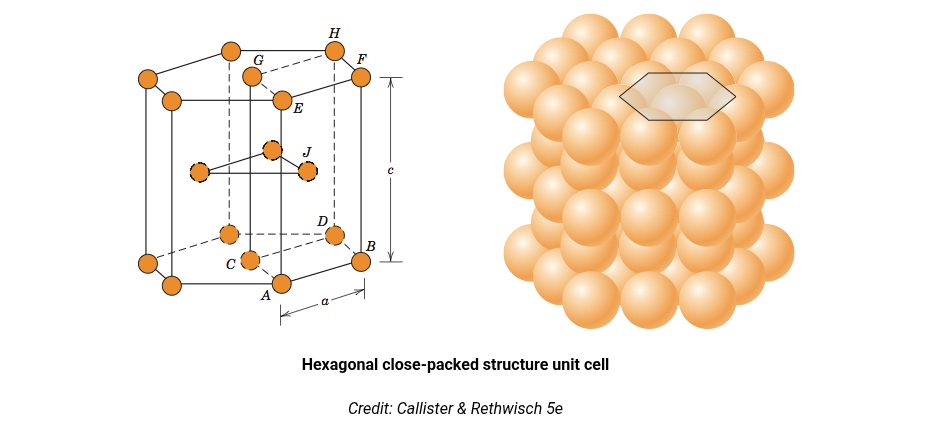
\includegraphics[width=0.75\textwidth]{hcp_celda.png}
\caption{\textbf{Celda unitaria de la estructura hexagonal compacta (HCP).}  
A la izquierda se muestra la celda convencional, caracterizada por los parámetros de red \(a\) (distancia basal entre centros de átomos) y \(c\) (altura de la celda).  
A la derecha se ilustra el apilamiento tridimensional de esferas duras en el patrón \emph{ABAB...}, donde cada átomo está rodeado por doce vecinos: seis en su mismo plano, tres en la capa superior y tres en la inferior.  
El contacto entre esferas ocurre tanto en el plano basal como entre capas, generando el empaquetamiento más denso posible.  
\textit{Fuente: Callister \& Rethwisch, 5e.}}
\label{fig:hcp}
\end{figure}

El \textcolor{Cerulean}{\textbf{factor de empaquetamiento}} en la estructura \textbf{hexagonal compacta (HCP)} se define, al igual que en las estructuras \textbf{SC}, \textbf{BCC} y \textbf{FCC}, como la fracción del volumen de la celda unitaria que está realmente ocupada por los átomos idealizados como esferas duras:

\begin{equation}
\begin{split}
\eta &= \frac{V_{\text{átomos en la celda}}}{V_{\text{celda}}}
\end{split} \label{eq:def-factor-hcp}
\end{equation}

El término \(V_{\text{átomos en la celda}}\) representa el volumen total ocupado por los átomos contenidos dentro de una celda unitaria, mientras que \(V_{\text{celda}}\) es el volumen geométrico de la misma.  
Ambas magnitudes se obtienen a partir de la geometría y del número efectivo de átomos que realmente pertenecen a la celda.

\vspace{0.4cm}

En la celda hexagonal convencional de la estructura HCP, el conteo efectivo de átomos es \underline{\(N_{\text{ef}}=6\)}.  
Esto se obtiene considerando que:
\begin{itemize}
  \item[$\bullet$] \(2\) átomos pertenecen completamente a la celda (uno en cada plano basal),
  \item[$\bullet$] \(12\) átomos en las esquinas del prisma aportan \(1/6\) cada uno, y
  \item[$\bullet$] \(3\) átomos están ubicados dentro del volumen central de la celda.
\end{itemize}
La suma de estas fracciones da como resultado un total equivalente a seis átomos completos por celda.

El volumen total ocupado por los átomos es entonces:

\begin{equation}
\begin{split}
V_{\text{átomos en la celda}} &= N_{\text{ef}}\;\frac{4}{3}\pi r^{3}
                              = 6\;\frac{4}{3}\pi r^{3}
                              = 8\pi r^{3}
\end{split} \label{eq:vol-atomos-hcp}
\end{equation}

Por otro lado, el volumen geométrico de la celda hexagonal se obtiene multiplicando el área del hexágono regular de base por la altura \(c\):

\begin{equation}
\begin{split}
V_{\text{celda}} &= \left(\frac{3\sqrt{3}}{2}\,a^{2}\right)c
\end{split} \label{eq:vol-celda-hcp}
\end{equation}

Aquí:
- \(a\) representa el parámetro de red basal (distancia entre centros de átomos en el plano inferior),  
- \(c\) es la altura de la celda unitaria, correspondiente a la distancia entre planos \emph{AB} consecutivos en el apilamiento \emph{ABAB...}.

\vspace{0.4cm}

En el \underline{empaquetamiento compacto ideal}, las esferas se encuentran en contacto tanto dentro de cada capa como entre capas adyacentes.  
Esta condición impone dos relaciones geométricas fundamentales:

\begin{itemize}
  \item[$\bullet$] En el plano basal, los átomos se tocan tangencialmente, por lo que \(a = 2r\).
  \item[$\bullet$] La proporción ideal entre la altura y la base está determinada por el contacto tridimensional entre las esferas:
  \[
  \frac{c}{a} = \sqrt{\frac{8}{3}}
  \]
\end{itemize}

Esta razón, conocida como \underline{relación ideal \(c/a\)}, garantiza que la tercera capa se acomode exactamente en los huecos formados por la primera y la segunda, evitando vacíos estructurales.

De la relación anterior y usando \(a = 2r\), se obtiene la altura \(c\) en función del radio atómico:

\begin{equation}
\begin{split}
c &= \sqrt{\frac{8}{3}}\,a = 2r\,\sqrt{\frac{8}{3}}
\end{split} \label{eq:c-en-r}
\end{equation}

Sustituyendo las ecuaciones \eqref{eq:vol-atomos-hcp}, \eqref{eq:vol-celda-hcp}, \(a=2r\) y \eqref{eq:c-en-r} en la definición general \eqref{eq:def-factor-hcp}, se tiene:

\begin{equation}
\begin{split}
\eta &= \frac{V_{\text{átomos en la celda}}}{V_{\text{celda}}}
     = \frac{8\pi r^{3}}{\left(\frac{3\sqrt{3}}{2}(2r)^{2}\right)\left(2r\sqrt{\frac{8}{3}}\right)}
     = \frac{8\pi r^{3}}{6\sqrt{3}\,r^{2}\,(2r)\sqrt{\frac{8}{3}}}
\end{split} \label{eq:eta-hcp-1}
\end{equation}

Simplificando los términos en \(r^{3}\) y desarrollando el denominador:

\begin{equation}
\begin{split}
\eta &= \frac{8\pi}{12\,\sqrt{3}\,\sqrt{\frac{8}{3}}}
     = \frac{8\pi}{12\,\sqrt{8}}
     = \frac{\pi}{3\sqrt{2}}
\end{split} \label{eq:eta-hcp-2}
\end{equation}

Por lo tanto, el \textcolor{Cerulean}{\textbf{factor de empaquetamiento}} para la estructura HCP es:

\begin{equation}
\begin{split}
\boxed{\eta_{\text{HCP}} = \frac{\pi}{3\sqrt{2}} \;\approx\; 0.740}
\end{split} \label{eq:eta-hcp-num}
\end{equation}

\vspace{0.3cm}

El resultado demuestra que:

\[
\boxed{\eta_{\text{HCP}} = \eta_{\text{FCC}} = 0.74}
\]

es decir, tanto la \textbf{estructura hexagonal compacta (HCP)} como la \textbf{cúbica centrada en las caras (FCC)} presentan el mismo grado de empaquetamiento máximo de esferas duras.  
La diferencia fundamental entre ambas radica en la \underline{secuencia de apilamiento}:  
en la FCC las capas se repiten como \emph{ABCABC...}, mientras que en la HCP lo hacen en el patrón \emph{ABAB...}.  

Ambas configuraciones logran el límite teórico de empaquetamiento más eficiente en tres dimensiones, con un \(74\%\) del volumen total ocupado por átomos y un \(26\%\) restante de huecos intersticiales.

Por consiguiente, la jerarquía global de densidad de empaquetamiento entre las estructuras cristalinas estudiadas es:

\[
\eta_{\text{SC}} = 0.52 \;<\;
\eta_{\text{BCC}} = 0.68 \;<\;
\eta_{\text{FCC}} = \eta_{\text{HCP}} = 0.74
\]

\noindent
De esta manera, la \textbf{HCP}, al igual que la \textbf{FCC}, se considera una red \underline{geométricamente óptima}, donde la disposición tridimensional de las esferas permite aprovechar al máximo el espacio disponible, cumpliendo el ideal del \emph{empaquetamiento compacto}.

	



\end{document}
